\paragraph{Game}

\begin{enumerate}

\item {\bf A 3-Player Game Tree} 

Consider the 3-player game shown below.  The player going first (at the top
of the tree) is the Left player, the player going second is the Middle
player, and the player going last is the Right player, optimizing the
left, middle and right components respectively of the utility vectors shown.   Fill in the
values at all nodes.  Note that all players \emph{maximize} their
own respective utilities.

\begin{center}
    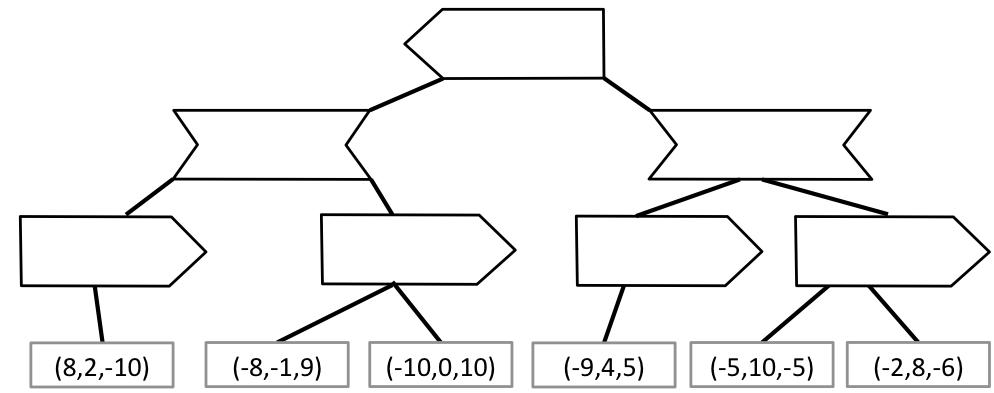
\includegraphics[width=4.5in]{figures/abg_q}
\end{center}

\vspace{1cm}


\item {\bf Pruning for a 3-Player Zero-Sum Game Tree}

We would like to prune nodes in a fashion similar to $\alpha$ - $\beta$ pruning.  Assume that we have the knowledge that the sum of the utilities of all 3 players is always zero.
What pruning is possible under this assumption?  Below, cross off with an $\times$ any branches that can be safely pruned.   If no branches can be pruned, justify why not:

\begin{center}
    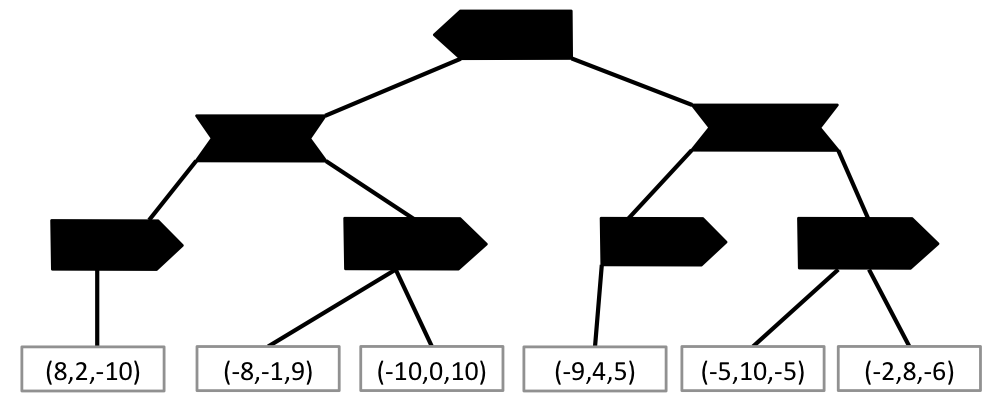
\includegraphics[width=4in]{figures/skeleton}
\end{center}

\vspace{5cm}


\item {\bf Pruning for a 3-Player Zero-Sum, Bounded-Utility Game Tree.}

If we assume more about a game, additional pruning may become possible.  Now, in addition to assuming that the sum of the utilities of
all 3 players is still zero, we also assume that all utilities are in the interval $[-10, 10]$.
What pruning is possible under these assumptions?  Below, cross off with an $\times$ any branches that can be safely pruned.   If no branches can be pruned, justify why not:

\begin{center}
    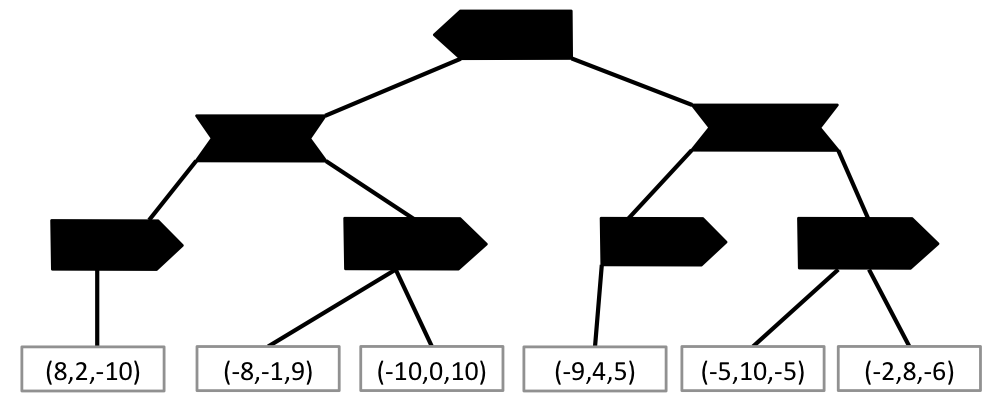
\includegraphics[width=4in]{figures/skeleton}
\end{center}

\end{enumerate}